\chapter{Einleitung}

\section{Optimierungsalgorithmen aus dem Bereich der Schwarmintelligenz}
Algorithmen aus dem Bereich der Schwarmintelligenz werden zur Optimierung von Problemen verwendet, in dem Verhaltensstrukturen aus der Natur mathematisch abgebildet und nutzbar gemacht werden.\\
Dabei wird versucht im Verhalten von Lebewesen Muster zu finden, mit denen ein Ziel erreicht werden kann, um somit die Zielfindung mathematischer Probleme zu optimieren. Gesucht wird dabei ein Optimum, also ein globales Minimum oder Maximum einer mehrdimensionalen mathematischen Funktion.\\
Der Algorithmus 'Elephant Herding Optimization' arbeitet rundenbasiert in Iterationen, wobei eine Obergrenze definiert werden kann.

\section{Elefanten} 
\begin{figure}[ht]
    \begin{center}
        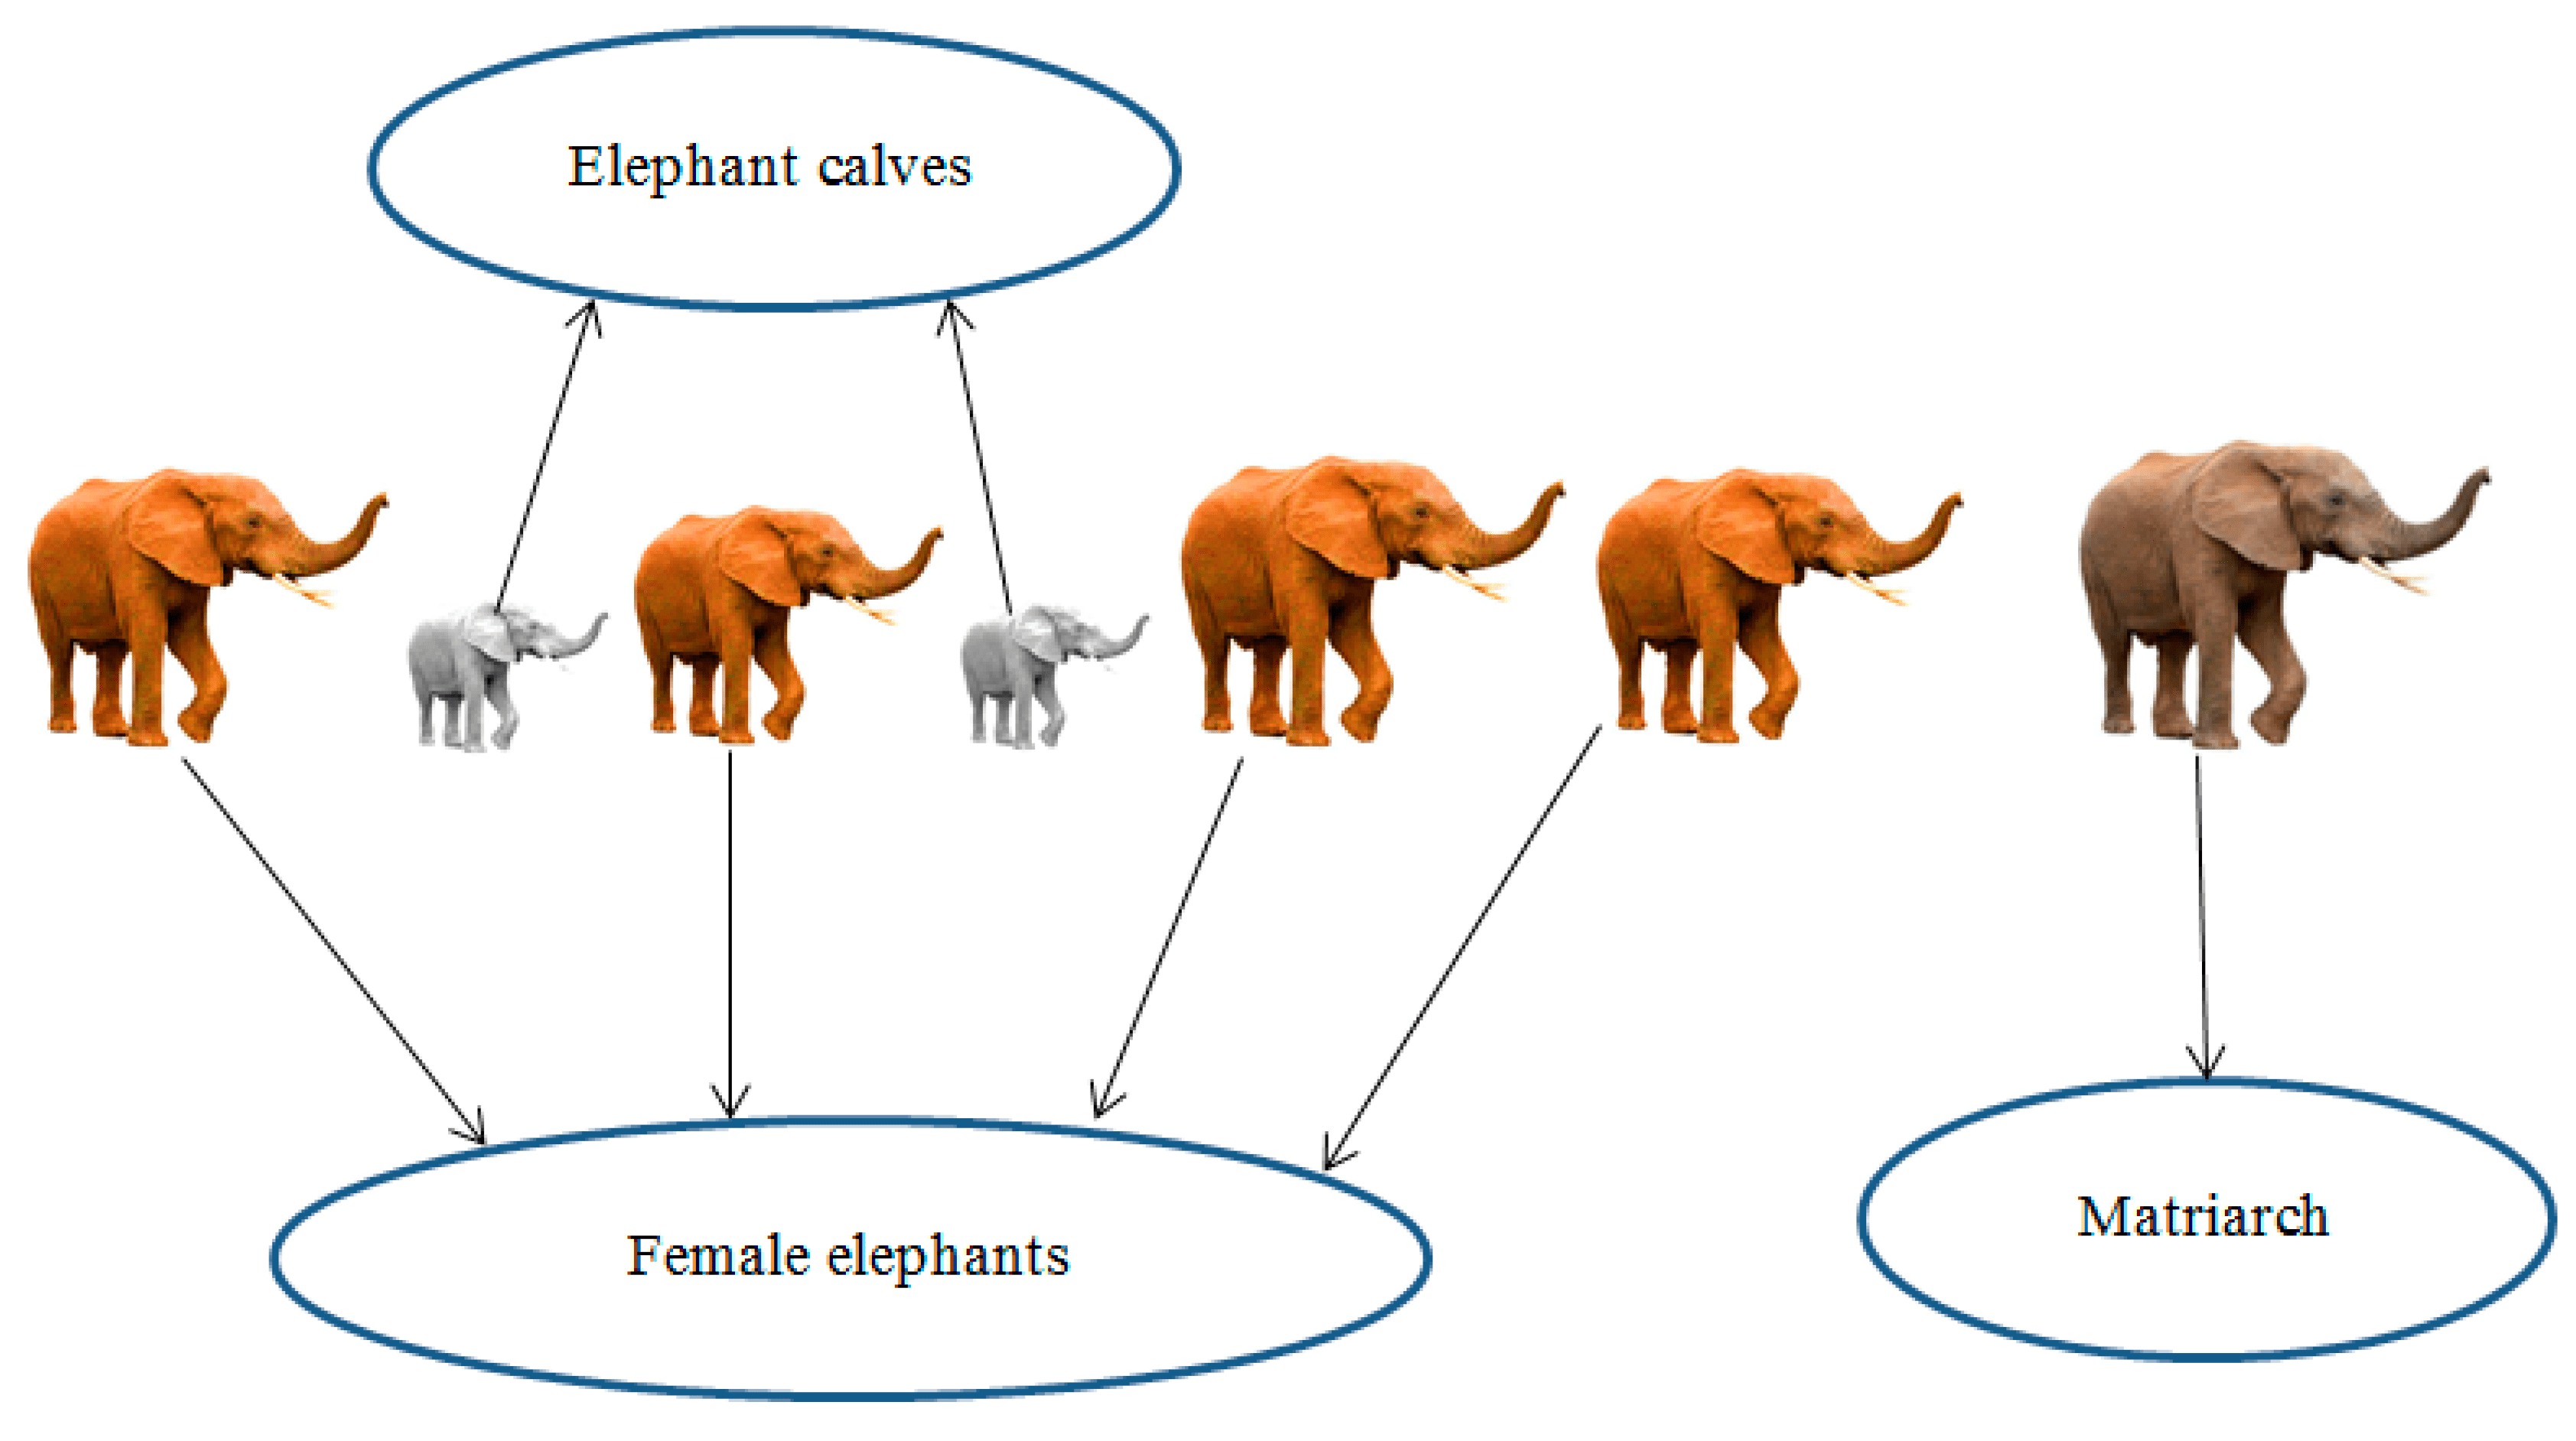
\includegraphics[width=0.7\textwidth]{assets/img/eho_socialstruct.png}
        \caption[EHO Social Structure in a clan]{\cite[Li et al, S.3]{li_lei_alavi_wang_2020}}
        \label{eho_socialstruct}
    \end{center}
\end{figure}
Elefanten sind soziale Tiere mit komplexen Sozialstrukturen. Eine Elefantenherde unterteilt sich in mehrere Clans, die aus weiblichen Tieren und ihren Jungtieren bestehen. Jeder Clan wird von einem Matriarch angeführt, der oft durch die älteste zugehörige Elefantenkuh repräsentiert wird, (siehe \autoref{eho_socialstruct}). Männliche Elefanten leben in Isolation und scheiden mit im Laufe ihres Heranwachsens aus dem Clan aus, \cite[vgl. Wang et al. 2015, S.1]{wang_deb_coelho_2015}. \\
Für den Algorithmus wird die Fortbewegung der Elefanten in Abhängigkeit von ihrem Clan und dem zugehörigen Matriarchen abgebildet und das Ausscheiden der männlichen Tiere aus einem Clan, \cite[vgl. Wang et al, S.1]{wang_deb_coelho_2015}. 

